\documentclass[9pt]{beamer}

\usepackage[utf8]{inputenc}
\usepackage[english]{babel}
\usepackage{adjustbox}

%\usepackage{preambles/ub}
\usepackage{preambles/mine}

\usepackage{subfiles}

\usetheme{Luebeck}

\AtBeginSection[]{
    \begin{frame}
        \vfill
        \centering
        \begin{beamercolorbox}[sep=8pt,center,shadow=true,rounded=true]{title}
            \usebeamerfont{title}\insertsectionhead\par%
        \end{beamercolorbox}
        \vfill
    \end{frame}
}
\AtEndDocument{
    \begin{frame}
        \vfill
        \centering
        \begin{beamercolorbox}[sep=8pt, center, shadow=ture, rounded=ture]{title}
            \usebeamerfont{title}\texttt{leave;}\\\texttt{ret;}
        \end{beamercolorbox}
        \vfill
    \end{frame}
}

\title{Binary exploitation}
\subtitle{Memory corruption}

\author{Oriol Ornaque Blázquez}

\begin{document}

\begin{frame}
\titlepage
\end{frame}

\begin{frame}
    \tableofcontents[hideallsubsections]
\end{frame}

\section*{Introduction}
\begin{frame}{Introduction and objectives}
    Objectives:
\begin{itemize}
    \item Be able to craft working exploits for common memory corruption vulnerabilities
    \item Analyze a real vulnerability and develop a Proof-of-Concept.
\end{itemize}
\end{frame}

\section{Stack overflows}

\subsection{Stack frame}
\begin{frame}{Stack frame}
    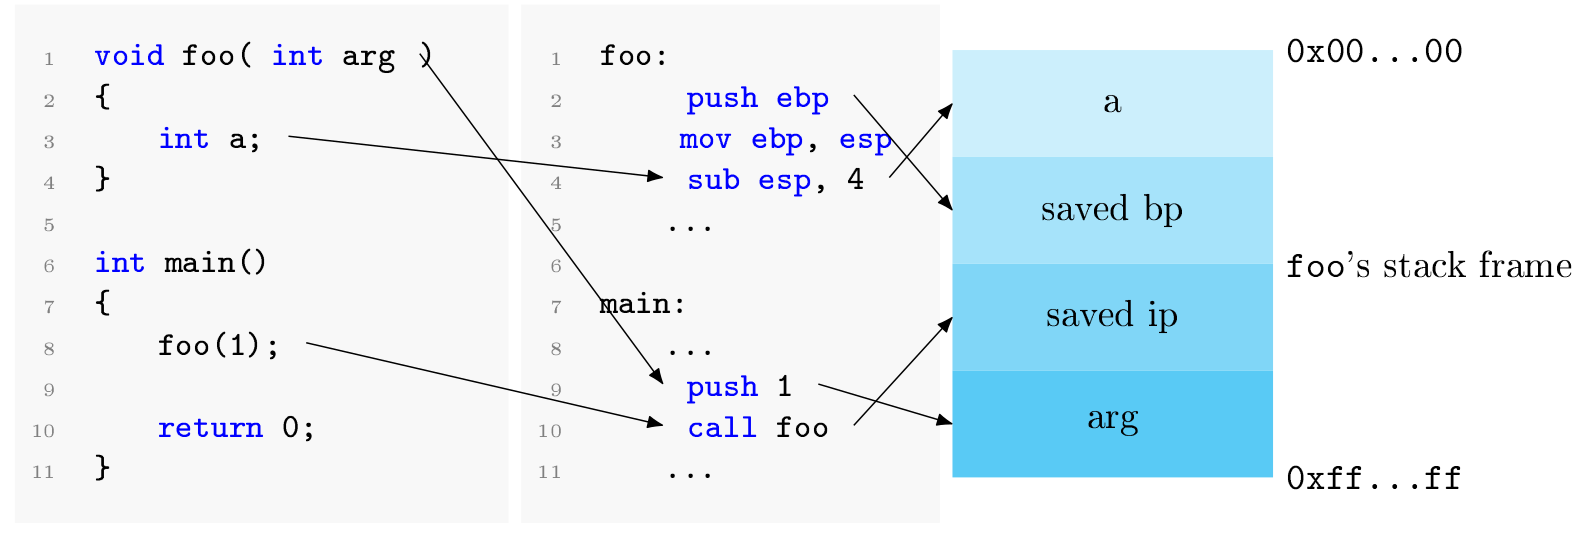
\includegraphics[width=\textwidth]{imgs/slides_extra/stack_frame.png}
\end{frame}

\subsection{Overwriting the return address}
\begin{frame}{Overwriting the return address}
\begin{adjustbox}{max totalsize={\textwidth}{0.5\textheight}, center}
\subfile{../imgs/stack_overflows/stack_buffer.tex}
\end{adjustbox}
\end{frame}

\subsection{Return into shellcode}
\begin{frame}{Return into shellcode}
    Place machine code into the stack buffer and return into it.
    \vspace{0.3cm}
\begin{adjustbox}{max totalsize={\textwidth}{0.5\textheight}, center}
    \subfile{../imgs/slides_extra/return_into_shellcode.tex}
\end{adjustbox}
\end{frame}

\section{Stack overflow countermeasures}

\subsection{Stack canaries}
\begin{frame}{Stack canaries}
    Place a random value after a buffer in the stack. When returning from a function check the integrity of that value. The value for the stack canary is generated at runtime everytime the binary is executed.\\
    \vspace{0.8cm}
\begin{adjustbox}{max totalsize={1\textwidth}{0.5\textheight}, center}
\subfile{../imgs/stack_overflow_counters/stack_canary.tex}
\end{adjustbox}
\end{frame}

\subsection{NX}
\begin{frame}{Non-executable memory}
    Mark memory sections as non-executable. If for some reason, the instruction pointer points to a non executable section, the program throws a segmentation fault and dies.

    \centering
    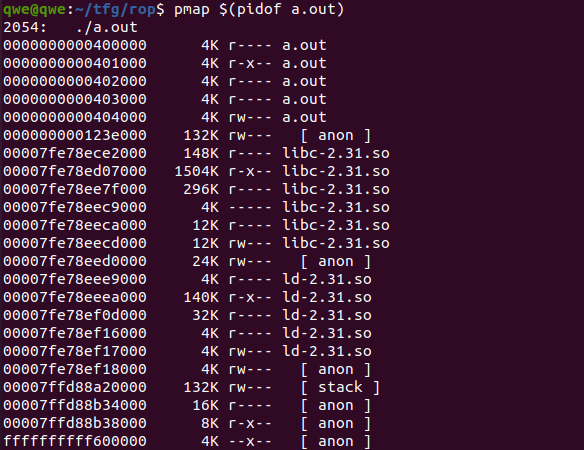
\includegraphics[height=0.6\textheight]{imgs/slides_extra/nx.png}
\end{frame}

\subsection{ASLR}
\begin{frame}{Address Space Layout Randomization}
Randomize the base address for all the sections in an executable at runtime. Everytime the binary is executed, the base addresses will change.\\
    \vspace{0.3cm}
    \centering
    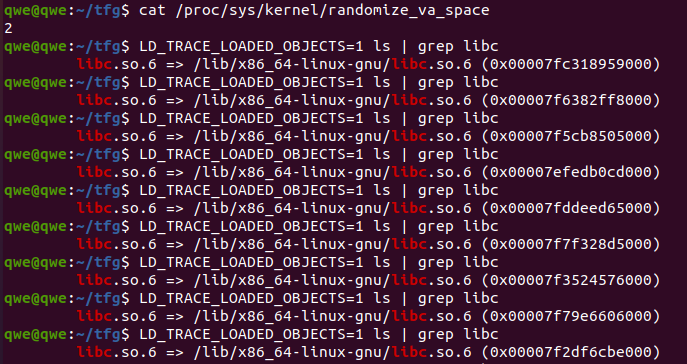
\includegraphics[scale=0.35]{imgs/stack_overflow_counters/addresses_aslr.png}
\end{frame}

\section{Format strings}

\subsection{Format strings}
\begin{frame}{Format strings}
    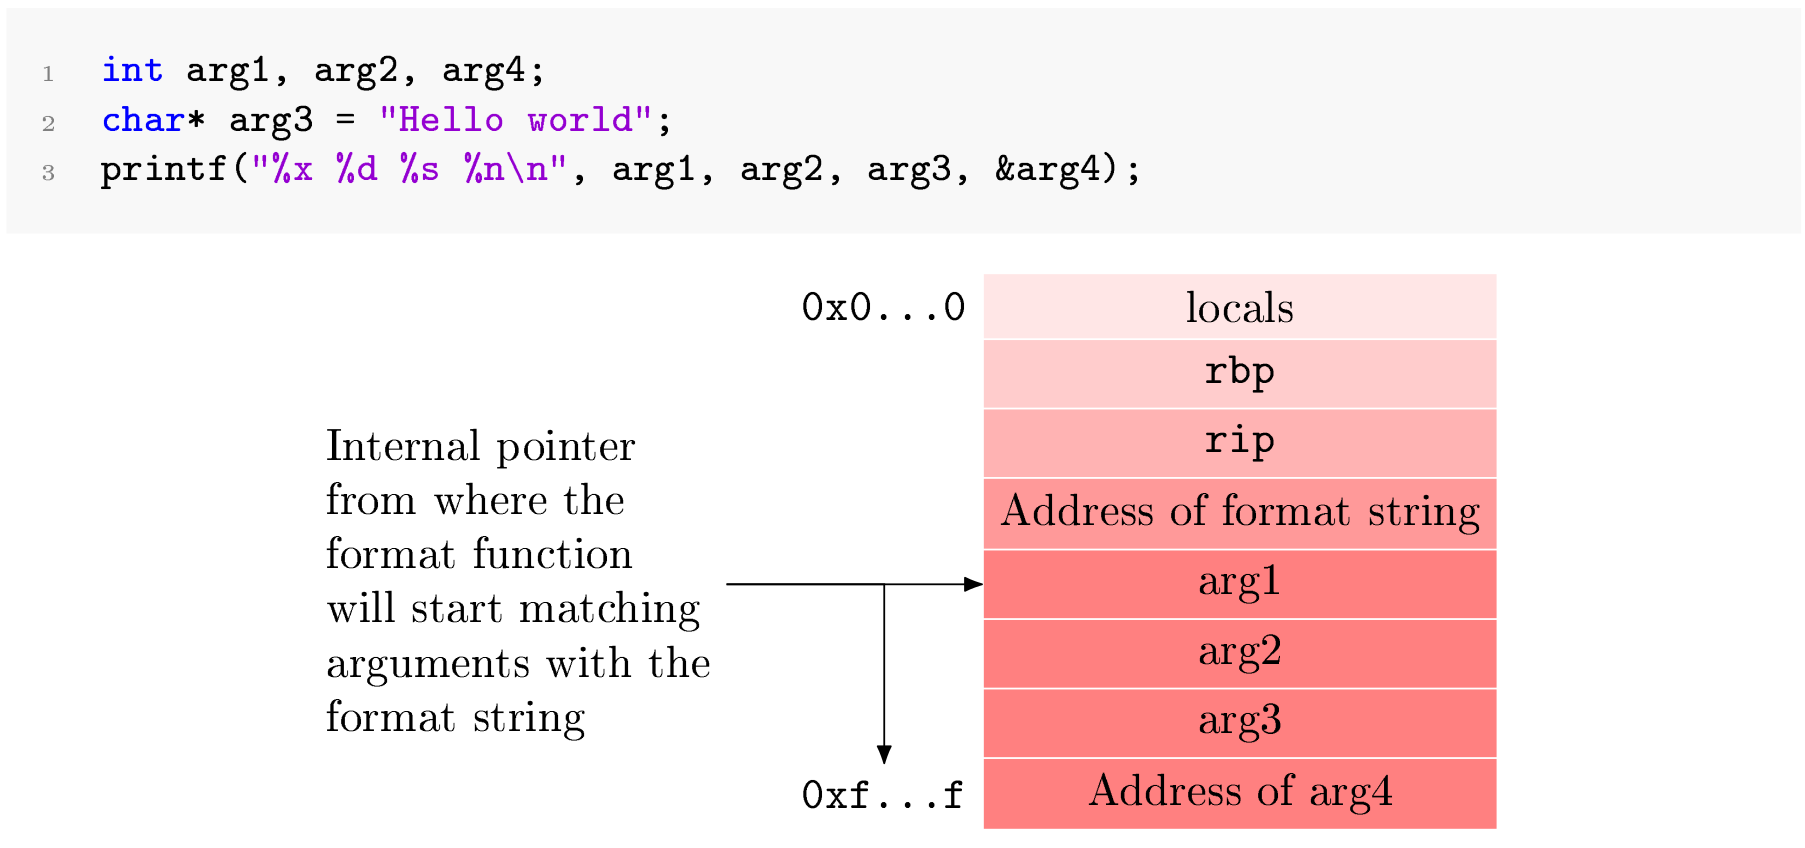
\includegraphics[width=\textwidth]{imgs/slides_extra/fmt_str_stack_frame.png}
\end{frame}

\subsection{Arbitrary read}
\begin{frame}{Arbitrary read}
\begin{adjustbox}{max totalsize={1\textwidth}{0.5\textheight}, center}
\subfile{../imgs/format_strings/arbitrary_read.tex}
\end{adjustbox}
\end{frame}

\subsection{Arbitrary write}
\begin{frame}{Arbitrary write}
\begin{adjustbox}{max totalsize={1\textwidth}{0.5\textheight}, center}
\subfile{../imgs/slides_extra/arbitrary_write.tex}
\end{adjustbox}
\end{frame}

\section{Return-oriented programming}

\subsection{ret2libc}
\begin{frame}{ret2libc}
    Return into the \texttt{system} function inside libc.
\begin{adjustbox}{max totalsize={1\textwidth}{0.5\textheight}, center}
\subfile{../imgs/rop/ret2libc_stack_layout.tex}
\end{adjustbox}
\end{frame}

\subsection{Return-oriented programming}
\begin{frame}{Return-oriented programming}
    Chain ROP gadgets to build a program.
\begin{adjustbox}{max totalsize={1\textwidth}{0.5\textheight}, center}
\subfile{../imgs/rop/rop_chain.tex}
\end{adjustbox}
\end{frame}

\subsection{Stack pivoting}
\begin{frame}[fragile]{Stack pivoting}
    Replacing the legitimate stack. Useful when there is no space for long ROP chains. Using the gadget \texttt{leave; ret} we can set the value for the stack pointer.
    \vspace{0.3cm}

    \begin{columns}
        \column{0.5\textwidth}
            The \texttt{leave} instruction is equivalent to:
\begin{lstlisting}
    mov rsp, rbp
    pop rbp
\end{lstlisting}
            Every function, except main, ends with \texttt{leave; ret}.
        \column{0.5\textwidth}
            \begin{adjustbox}{max totalsize={1\textwidth}{0.5\textheight}, center}
            \subfile{../imgs/rop/stack_pivot_stack.tex}
            \end{adjustbox}
    \end{columns}

\end{frame}

\subsection{ret2dlresolve}
\begin{frame}{ret2dlresolve: resolving dynamic symbols}
    \centering
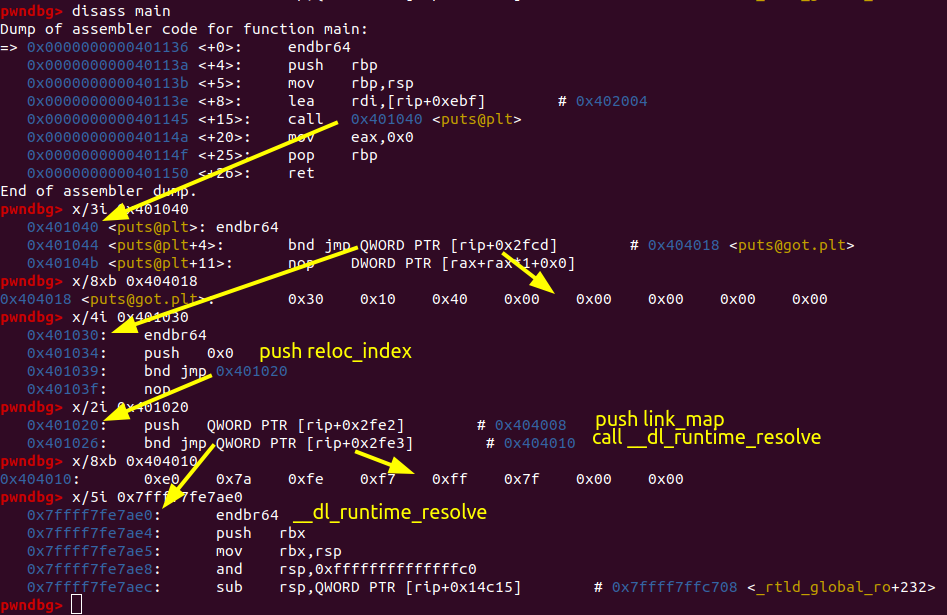
\includegraphics[scale=0.38]{imgs/rop/ret2dlresolve/plt_got_dlresolve.png}
\end{frame}

\begin{frame}{ret2dlresolve: structures}
    \begin{columns}
        \column{0.6\textwidth}
            JMPREL maps a symbol to an offset on the GOT. The \texttt{r\_info} field gives us the index  of the symbol on the SYMTAB.\\
            \vspace{0.3cm}
            SYMTAB stores information about the symbols. The most important field for this exploit is \texttt{st\_name} which is the offset on the STRTAB structure.\\
            \vspace{0.3cm}
            STRTAB is a table of null terminated strings. Stores the name of the symbols.\\
        \column{0.4\textwidth}
            \begin{adjustbox}{max totalsize={1\textwidth}{0.5\textheight}, center}
                \subfile{../imgs/rop/ret2dlresolve_structures.tex}
            \end{adjustbox}
    \end{columns}
\end{frame}

%\begin{frame}{ret2dlresolve: memory layout}
    %\begin{adjustbox}{max totalsize={1\textwidth}{0.5\textheight}, center}
        %\subfile{../imgs/rop/ret2dlresolve/offsets.tex}
    %\end{adjustbox}
%\end{frame}

\subsection{Sigreturn oriented programming}
\begin{frame}{Sigreturn oriented programming}
\begin{adjustbox}{max totalsize={1\textwidth}{0.7\textheight}, center}
\subfile{../imgs/rop/srop/srop_layout.tex}
\end{adjustbox}
\end{frame}

\section{Heap exploitation}

\subsection{Heap data structures}
\begin{frame}{ptmalloc's chunk}
    \begin{columns}
        \column{0.5\textwidth}
            \begin{adjustbox}{max totalsize={1\textwidth}{0.5\textheight}, center}
                \subfile{../imgs/heap_exploits/allocated_chunk_struct.tex}
            \end{adjustbox}
        \column{0.5\textwidth}
            \begin{adjustbox}{max totalsize={1\textwidth}{0.5\textheight}, center}
                \subfile{../imgs/heap_exploits/freed_chunk_struct.tex}
            \end{adjustbox}
    \end{columns}
\end{frame}

\begin{frame}{glibc's tcache}
\begin{adjustbox}{max totalsize={1\textwidth}{0.5\textheight}, center}
\subfile{../imgs/heap_exploits/tcache_struct.tex}
\end{adjustbox}
\end{frame}

\subsection{Heap overflow}
\begin{frame}{Heap overflow}
\begin{adjustbox}{max totalsize={1\textwidth}{0.5\textheight}, center}
\subfile{../imgs/heap_exploits/heap_overflow.tex}
\end{adjustbox}
\end{frame}

\subsection{UAF}
\begin{frame}{UAF}
    \centering
        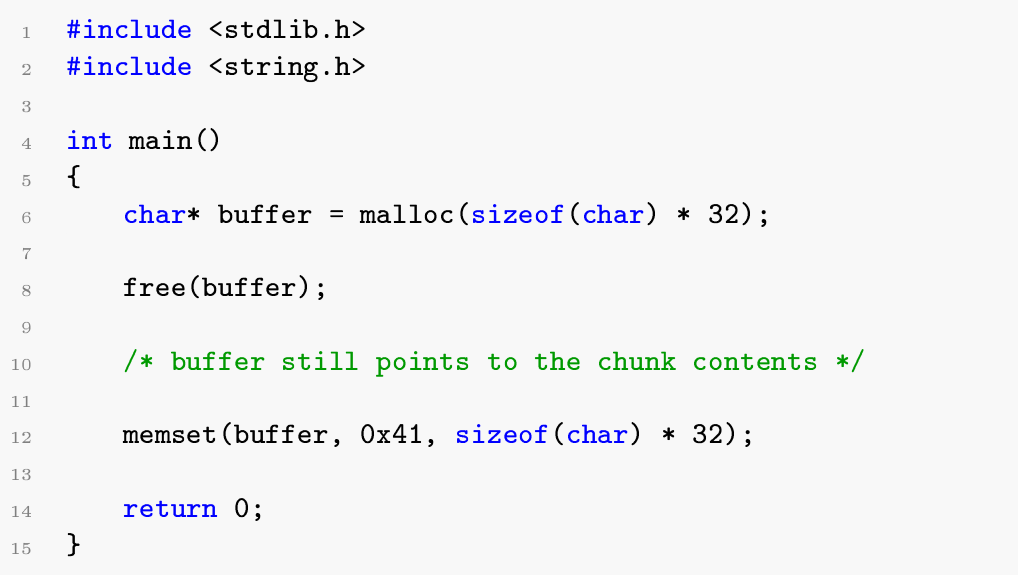
\includegraphics[scale=0.35]{imgs/slides_extra/uaf.png}
\end{frame}

\subsection{Double free}
\begin{frame}{Double free}
    \centering
    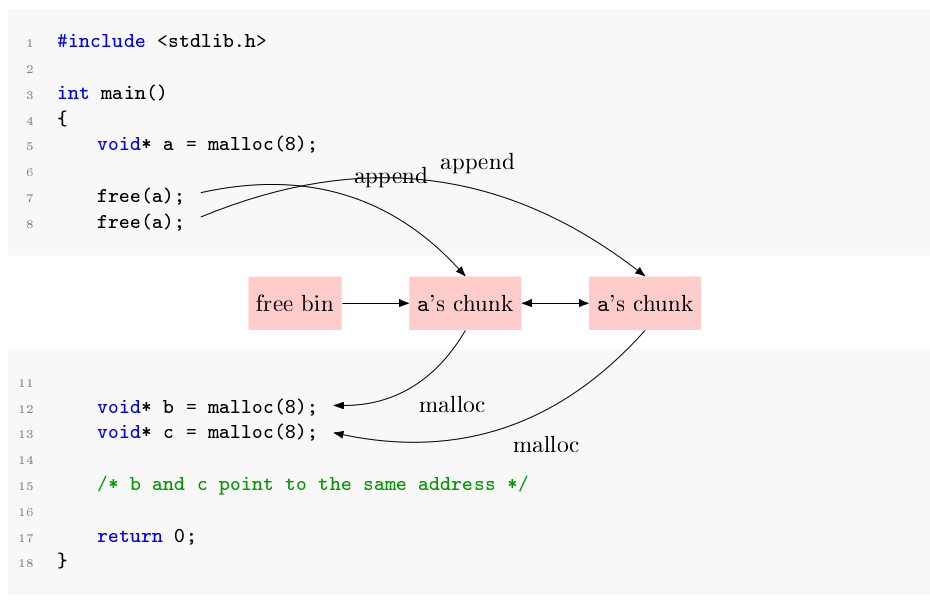
\includegraphics[scale=0.4]{imgs/slides_extra/double_free.png}
\end{frame}

\subsection{Unlink}
\begin{frame}{Unlink}
    \begin{columns}
        \column{0.5\textwidth}
        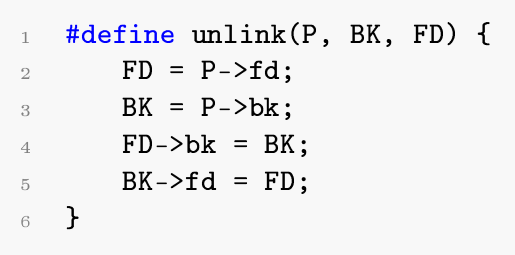
\includegraphics[scale=0.4]{imgs/slides_extra/unlink_macro.png}
        \column{0.5\textwidth}
        \begin{adjustbox}{max totalsize={1\textwidth}{0.5\textheight}, center}
            \subfile{../imgs/heap_exploits/unlink/controlled_chunk.tex}
        \end{adjustbox}
    \end{columns}
    \vspace{0.3cm}
    \begin{centering}
    \texttt{FD} $=$ \texttt{0x5655d804}\\
    \texttt{BK} $=$ \texttt{0x5508f311}\\
    *(\texttt{0x5655d804} $+$ \texttt{0xc}) $=$ \texttt{0x5508f311}\\
    *(\texttt{0x5508f311} $+$ \texttt{0x8}) $=$ \texttt{0x5655d804}\\
    \end{centering}
\end{frame}

\section{Fuzzing}

\subsection{Fuzzing}
\begin{frame}{Fuzzing}
Automatically generate test cases for the program with the intention to find vulnerabilities.
    \begin{itemize}
        \item Very popular technique.
        \item Great quality open source tools that have proven their worth: \emph{afl}, \emph{Hongfuzz}, \emph{libFuzz}, ...
        \item Used and trusted by tech leading companies:
            \begin{itemize}
                    \item Google: OSS-Fuzz project.
                    \item Microsoft: OneFuzz project.
            \end{itemize}
    \end{itemize}
    \vspace{0.3cm}

    \centering
        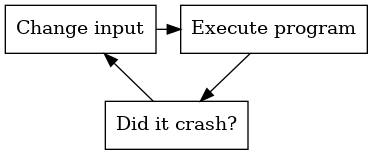
\includegraphics[scale=0.4]{imgs/slides_extra/fuzzing_loop.png}
\end{frame}

%\begin{frame}{Types of fuzzers}
    %\begin{itemize}
            %\item Input seed
                %\begin{itemize}
                        %\item Generative
                        %\item Mutation-based
                %\end{itemize}
            %\item Input structure
                %\begin{itemize}
                    %\item Unstructured
                    %\item Structured
                %\end{itemize}
            %\item Program knowledge
                %\begin{itemize}
                        %\item Blackbox
                        %\item Whitebox
                        %\item Greybox
                %\end{itemize}
    %\end{itemize}
%\end{frame}

\section{CVE-2021-3156 PoC}

\subsection{CVE-2021-3156}
\begin{frame}{CVE-2021-3156}
    Nicknamed Baron Samedit. Disclosed by Qualys Research Team on 26/01/2021. Affected the \texttt{sudo} program.
    \begin{itemize}
        \item Priviledge escalation to root.
        \item Heap overflow caused by an off-by-one error
        \item Affected versions:
            \begin{itemize}
                    \item 1.8.2-1.8.31p2 for legacy versions
                    \item 1.9.0-1.9.5p1 for stable versions.
            \end{itemize}
        \item The commit that created the vulnerability was merged on 2011
    \end{itemize}
\end{frame}

\begin{frame}{Sudo's overview}
    \begin{columns}
        \column{0.6\textwidth}
            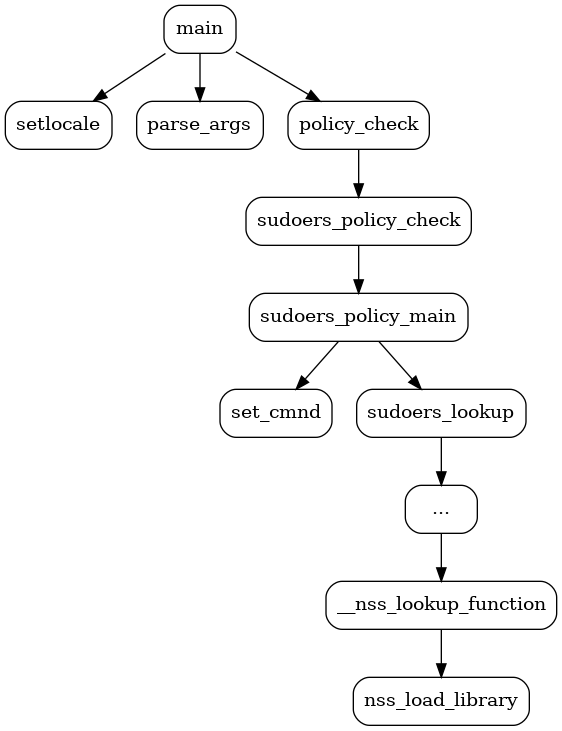
\includegraphics[scale=0.2]{imgs/examples/baron_samedit/call_graph.png}
        \column{0.4\textwidth}
            \begin{itemize}
                \item[\texttt{setlocale}]: sets the locale in accordance with \texttt{LC\_*} environment variables.
                \item[\texttt{parse\_args}]: escapes metacharacters from the command line arguments arguments.
                \item[\texttt{set\_cmnd}]: copies the command line arguments to a heap buffer. The overflow happens here.
                \item[\texttt{nss\_load\_library}]: loads a library to fullfill a lookup.
            \end{itemize}
    \end{columns}
\end{frame}

%\subsection{Sudo's modes}
%\begin{frame}{Sudo's modes}
    %\texttt{parse\_args} escapes metacharacters, including backslashes. The input that causes the overflow require backslashes and therefore these function must not be called.
    %The condition to execute \texttt{set\_cmnd} but not \texttt{parse\_args} is:
%$$ \texttt{MODE\_SHELL} \wedge (\texttt{MODE\_EDIT} \vee \texttt{MODE\_CHECK}) \wedge \neg \texttt{MODE\_RUN}$$
%
    %Running \texttt{sudoedit} instead of \texttt{sudo} sets the \texttt{MODE\_EDIT} flag without the \texttt{MODE\_RUN} flag.
    %Using the option \texttt{-s} sets the \texttt{MODE\_SHELL} flag.
%\end{frame}

\subsection{Baron Samedit's overflow}
\begin{frame}{Baron Samedit's overflow}
    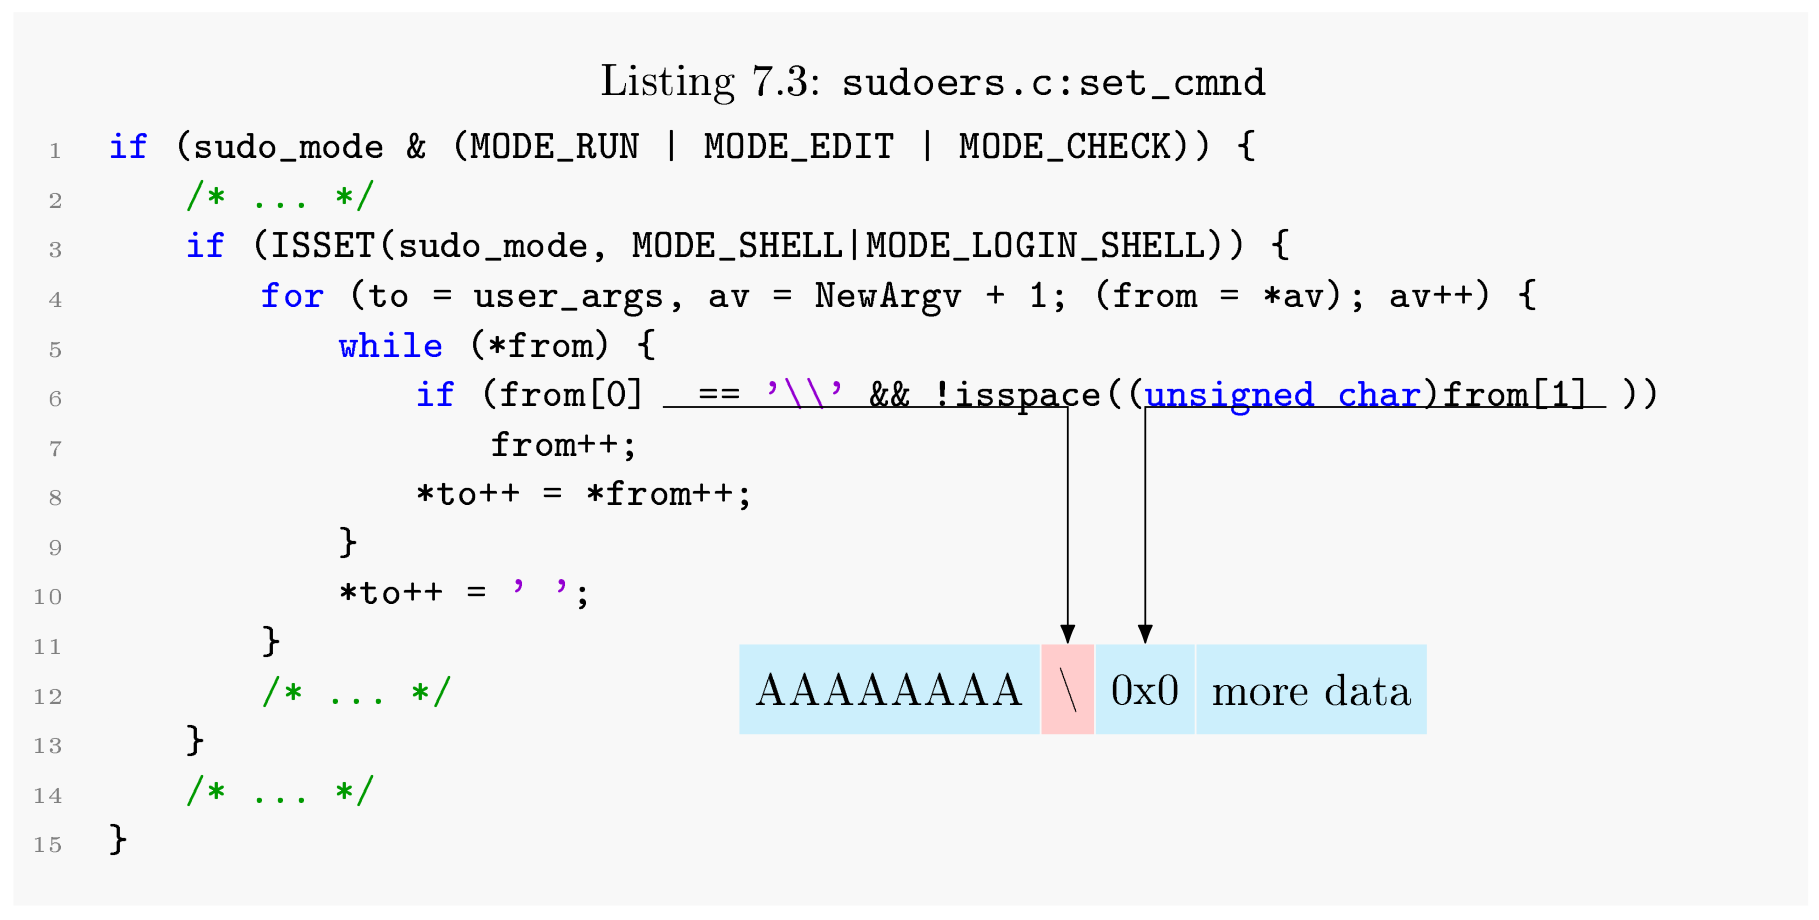
\includegraphics[width=\textwidth]{imgs/slides_extra/cve_overflow.png}
\end{frame}

\subsection{NSS}
\begin{frame}{Name Service Switch}
    \begin{columns}
        \column{0.5\textwidth}
            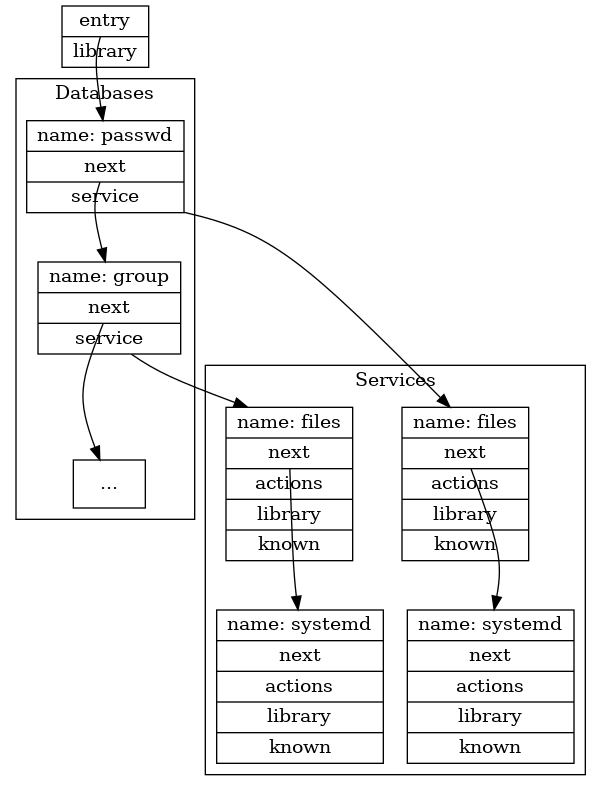
\includegraphics[scale=0.2]{imgs/examples/baron_samedit/nss_structs.png}
        \column{0.5\textwidth}
            Library to resolve information related to names.
            \texttt{sudo} uses it to check if a user belongs to the \texttt{sudo} group.\\

            We can use the overflow to change the name of the library loaded for one controlled by us.
    \end{columns}
\end{frame}

\subsection{Heap feng shui}
\begin{frame}{Heap feng shui}
    \begin{columns}
        \column{0.6\textwidth}
        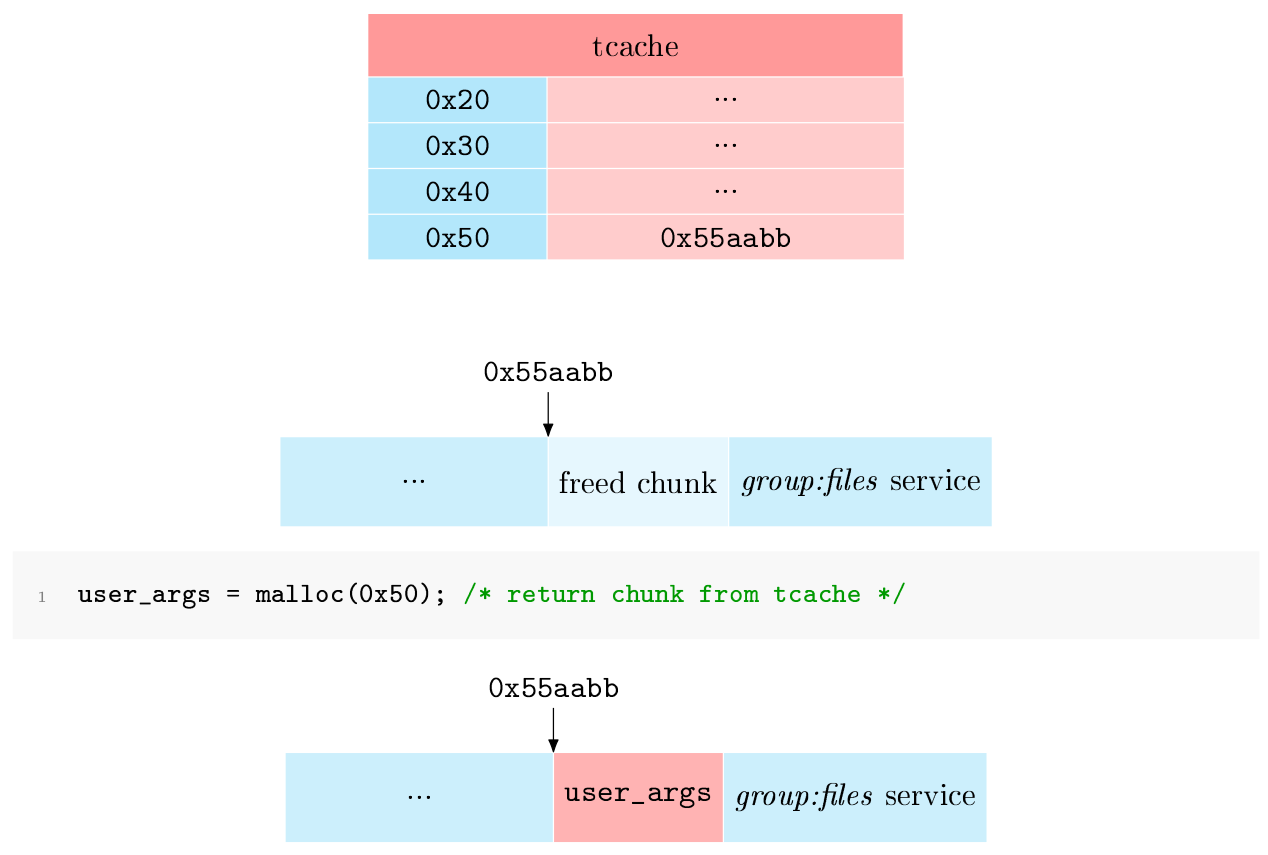
\includegraphics[scale=0.2]{imgs/slides_extra/heap_feng_shui.png}
        \column{0.4\textwidth}
        By doing allocations of certain sizes we can influence the overall heap layout.

        \texttt{setlocale} does a lot of allocations with the environment variables \texttt{LC\_*}. We can bruteforce the length of these variables to achieve a heap layout that benefits us.

    \end{columns}
\end{frame}

\begin{frame}{Heap feng shui}
    \begin{columns}
        \column{0.5\textwidth}
            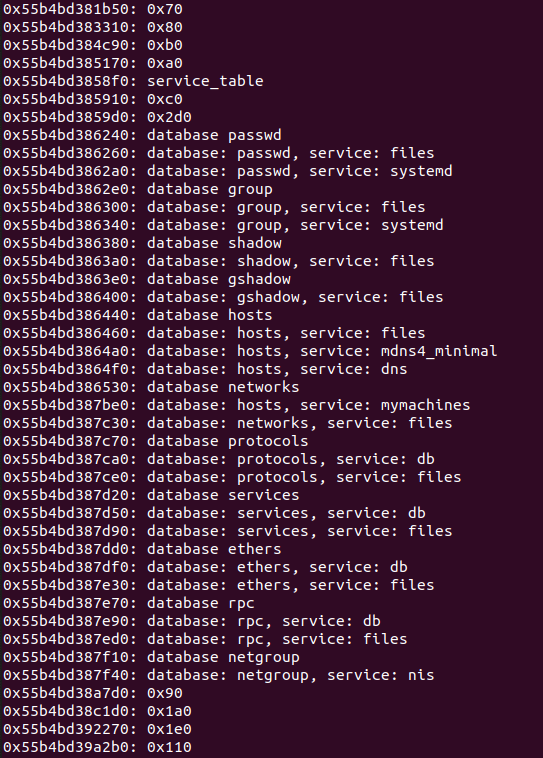
\includegraphics[scale=0.3]{imgs/examples/baron_samedit/brute_1.png}
        \column{0.5\textwidth}
            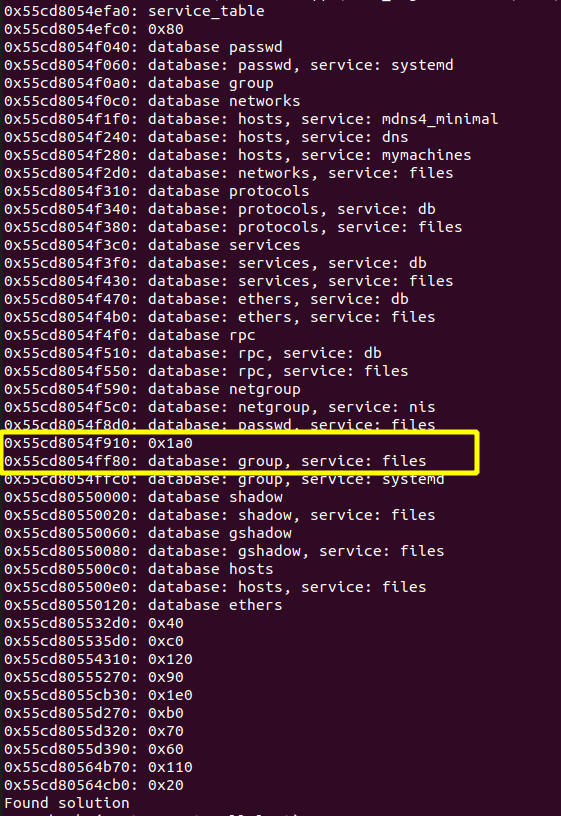
\includegraphics[scale=0.28]{imgs/examples/baron_samedit/brute_2.png}
    \end{columns}
\end{frame}

\subsection{Overwriting with environment variables}
\begin{frame}{Overwriting with environment variables}
    \centering

        \begin{adjustbox}{max totalsize={1\textwidth}{0.5\textheight}, center}
            \subfile{../imgs/examples/baron_samedit/overflow.tex}
        \end{adjustbox}
        \vspace{0.3cm}
    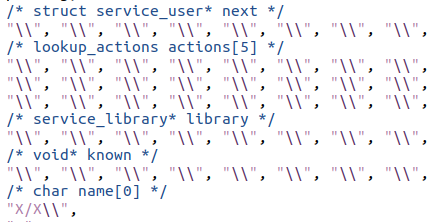
\includegraphics[scale=0.6]{imgs/slides_extra/env_overwrite.png}
\end{frame}

\subsection{Demo}
\begin{frame}{Demo}
    \centering
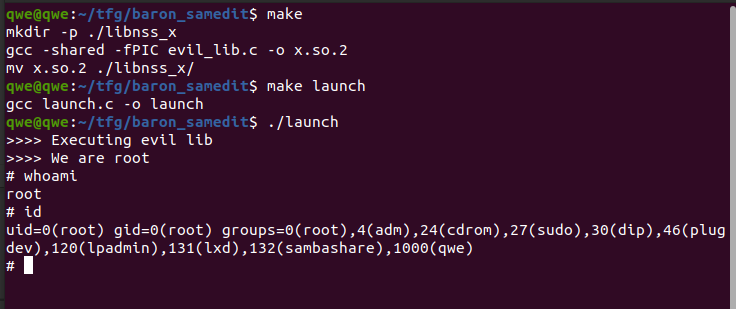
\includegraphics[width=\textwidth]{imgs/examples/baron_samedit/success.png}
\end{frame}

\end{document}
